\newpage
\section{Causal Discovery using Order-Informed Context}
\label{chapter:methodcontext}

% SECTIONS
% LCD/ICP
% Design of context variables and justification of decisions
% Assumptions and justification
% Short validation of synthetic data

\subsection{Local Causal Discovery}

% intro
Local Causal Discovery (LCD) was originally proposed by \citet{cooper1997simple} as a fast, incomplete algorithm. It can determine a direct causal relationship between two variables in a system of three variables. It can also be applied to a larger system by marginalizing over variable triples and testing for ancestral relationships between variables. 

% motivation
LCD is chosen as the causal inference method in this thesis because it is simple, and a good trade-off between performance and computation time. It was applied to the \citet{kemmeren2014large} dataset by \citet{versteeg2019boosting}. They compared LCD to ICP \citep{peters2016causal}, presenting a somewhat higher precision in the top predictions with ICP, at the cost of three times the computation time. 

\subsubsection{Assumptions}

The algorithm tests a causal relation $X\to Y$ between two endogenous variables, using a third exogenous variable $C$ (the context). A small set of statistical independence tests restricts the set of possible causal subgraphs with nodes $X$, $Y$ and $C$. Under some circumstances, it allowes us to infer  that $X$ is an ancestor of $Y$.

LCD relies on some assumptions. Like many inference algorithms, the starting point is to model the underlying system as a SCM. The context variable needs to be exogenous, such that no system variable can be its cause. Causal faithfulness is assumed to link (in)dependences to the d-separation of variables. To measure these (in)dependences from the data, the dependence and independence tests are taken as oracles, such that their outcomes are taken as the truth. Unbiased data selection and acyclicity are also assumed. 

\citet{mooij2016joint} show that the acyclicity assumption can be dropped if we adopt a different notion of separation called $\sigma$-separation. We will leave this topic at this note, because the theoretical properties of the LCD method are not the focus of this thesis.

\subsubsection{Statistical tests}

LCD discovers those causal relations, which effect can be measured from the data as $\Prb _M(Y|do(X=x)) = \Prb _M(Y|X=x)$. This is the case when there is no confounding between $X$ and $Y$, no effect of $Y$ on $X$, and no effect of $C$ on $Y$ that bypasses $X$. Figure \ref{fig:5:lcdgraphs} shows the three subgraphs that satisfy the condition. Note that all possible relations between $C$ and $X$ given the exogeneity assumption are allowed.

\begin{figure}[h]
    \centering
    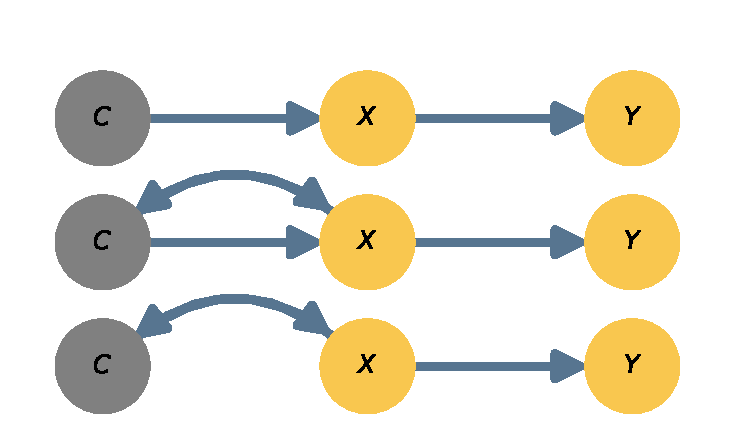
\includegraphics[width=.6\textwidth]{5LCDgraphs.pdf}
    \caption{All mixed graphs in which LCD can infer the relation $X\to Y$}
    \label{fig:5:lcdgraphs}
\end{figure}

All subgraphs satisfy one independence and five dependence relations:

% \setlist{nolistsep}
\begin{enumerate}[noitemsep]
    \item $C \CI Y \given X $
    \item $C \nCI Y$
    \item $C \nCI X$ (optional)
    \item $X \nCI Y$ (optional)
    \item $X \nCI Y \given C$ (optional)
    \item $C \nCI X \given Y$ (optional)
\end{enumerate}

\citet{cooper1997simple} proved that relations 1, 3, and 4 are sufficient to infer the causal relation $X\to Y$, by enlisting all possible subgraphs. \citet{versteeg2019boosting} only used relations 1 and 2, which are also sufficient.

Most LCD implementations only check two or three relations. However, if assumptions are violated or the dataset is small, some nonexistent causal relations might be inferred. One can sacrifice recall for precision by testing some or all of the remaining relations. \citet{cooper1997simple} warns specifically that the independence relation ($C \CI Y \given X$) is vulnerable to faithfulness violations, and suggests testing the second relation ($C \nCI Y$) as well. \citet{triantafillou2017predicting} aim for high precision and test all six relations.

A common choice of independence test is the two-tailed Fisher z-test \citep{fisher1924distribution}, which tests if the partial correlation is zero. In the application of this thesis, this test may be limited, since the context variable is constructed to have only two discrete values. As an intuitive example, we test the relation $C\nCI X$. The mean of $X$ given $C=0$ happens to be close to the mean given $C=1$. This makes it very hard to significantly show a correlation between $C$ and $X$. 

As a potentially better alternative, we use the mean-variance test that is used by \citet{versteeg2019boosting}, testing both the means and the variances across context values. The example given above would not fool this test, because there is a difference in variance. Regardless of this intuition, it should be noted that \citet{versteeg2019boosting} show hardly any difference in results due to the test.

When the test rejects the null hypothesis, we conclude (conditional) dependence between the variables. Reversely, when the test fails to reject the null hypothesis, we conclude (conditional) independence. We accept this dubious method, because it is simple and common in the causality field. We further follow the work of \citet{versteeg2019boosting} by choosing a different significance level for testing the dependence (2) and conditional independence (1) relation. The conditional independence test is made more strict by correcting for multiple testing, with an $\alpha_{indep}=\frac{0.01}{6182}$. It is not as straightforward to correct the test for the dependence relation, since we draw a conclusion when we fail to reject the hypothesis. Therefore, the significance level is kept at $\alpha_{dep}=0.01$.


\subsection{Context Design}

The \citet{kemmeren2014large} dataset does not provide clear context variables that are known to be exogenous. Therefore, the modeler can determine how to construct a context variable. Any context that is not informed by the values of the data is allowed, but some designs may be more productive than others. Recall that LCD is sound but not complete. A bad choice of context could result in a low recall. 

We can look at context design from the perspective of three sufficient LCD conditions. $X\nCI Y$ says that LCD only considers relations where dependence between $X$ and $Y$ is shown. This condition is irrelevant for context design. $C\nCI X$ means that we should choose the context such that it is expected to depend on $X$. In the case of a single binary context variable, we want the distribution of $X$ to be different depending on the value of $C$. Lastly, $C\nCI Y|X$ tells us that any dependence between the context and our potential target $Y$ should disappear once we know the value of $X$. 

Any background knowledge about the data can be used for the context. However, the sparsity of the data makes this task complicated. We would like to encode the target gene of interventions in a categorical context variable. However, there would only be one data point per context value, rendering independence testing impossible. The challenge is to generalize this information.

\subsubsection{Original Context Design}

The context used by \citet{versteeg2019boosting} is the ultimate generalization of the intervention target information. They introduce a single binary context variable that encodes if the data point is interventional or observational. 

Generally, when a gene is knocked out in the system, a different SCM is induced with a different distribution of the variables values. However, the effect of single interventions is typically restricted to a small number of genes that are significantly affected. When we are interested in the effects of some variable $X$, there may be some intervention data points where $X$ deviates from its normal value due to intervention on itself or its ancestors. However, the significance of these data points may be obfuscated by the large number of intervention data points where $X$ has a normal value. The clusters for $C=0$ and $C=1$ could be hardly distinguishable. 

% Moreover, the effectiveness of this context variable is questionable. Take the example in Figure \ref{fig:5:origlcd} of a Markov chain with variables $X_i$. Let's introduce binary intervention variables $I_i$ that equal $1$ if there is an intervention on $X_i$. We could describe the causal mechanism as $X_i = f(X_{i-1}, I_i)$. The context is then a function of all $I_i$. Specifically, $C=\bigcup I_i$ if we consider the values to be boolean. When we represent this graphically, we see that $C$ can act as a confounder between any variable pair. Although the exogeneity assumption is still satisfied, this confounding breaks the LCD condition $C\CI Y|X$. Concretely, when we try to prove the true relation $X_i\to X_j, i<j$, any data point with an intervention on $X_k, i<k\leq j$ disproves the conditional independence. This insight can be generalized to any acyclic graph with ordered nodes $X_i$. 

% \begin{figure}[h]
%     \centering
%     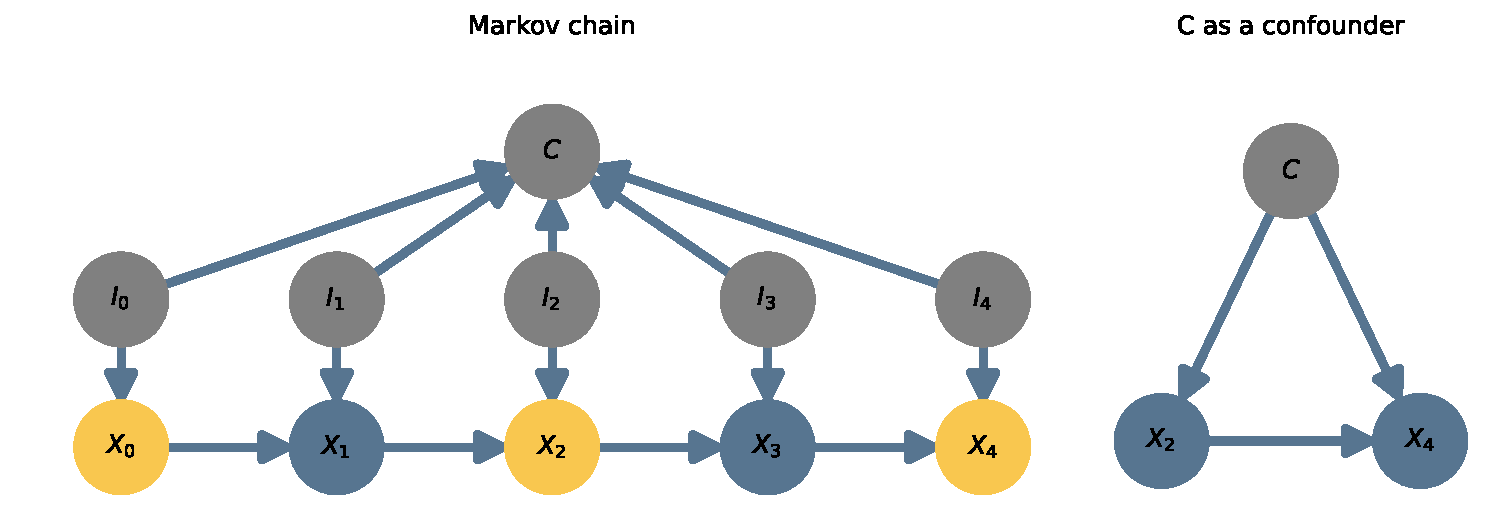
\includegraphics[width=\textwidth]{5origlcd_marginal.pdf}
%     \caption{Graphical representation of the LCD context as constructed by \citet{versteeg2019boosting} applied to a Markov chain, and its marginalization over the three relevant variables.}
%     \label{fig:5:origlcd}
% \end{figure}
 

\subsubsection{Order-based Context Design}

We hypothesize that a more specific context is more effective. Given a variable pair $(X,Y)$, the original context makes a distinction whether there is an intervention anywhere in the system. Most of these interventions don't even affect $X$ or $Y$. We would like a context that makes a distinction between an environment with an intervention that affects $X$, and an environment without such intervention. 

To construct a context based on this idea, we require two adaptations. First, for each variable $X$ we have a separate context variable $C_X$ that we use to test the relation $X\to Y$. Second, we need to estimate whether a given intervention is expected to affect $X$. 

The approach in this thesis is to estimate a causal order of the variables. Assuming acyclicity, interventions on genes later in the order than $X$ cannot affect it. Thus, we set the context to $1$ only if the intervention target is earlier in the order than $X$, or if $X$ is intervened on. 

Formally, we look at variable pairs $X_i, X_j$, and test the causal relation $X_i\to X_j$. For each variable $X_i$, we have some observation data points and intervention data points, such that $X_i = (X^O_i, X^I_i)$. The elements of the intervention data points $(X^I_i)_k$ are indexed according to the variable that is intervened on. For example, the intervention on $X_i$ itself is $(X^I_i)_i$. The inferred variable order is represented by a permutation $\pi$, such that $\pi_i$ indicates the position of variable $i$. We now construct the context $C_{X_i} = (C^O_{X_i}, C^I_{X_i})$ as follows.

$$\begin{array}{ll}
(C^O_{X_i})_k & =0 \\
(C^I_{X_i})_k & = \begin{cases}
    1 \text{ if } \pi_k\leq \pi_i \\
    0 \text{ if } \pi_k> \pi_i    
\end{cases}
\end{array}$$

Before we move to the experiments detailed in the next chapter, there is one problem that remains to be tackled. When we wish to predict the effects of variable $X_i$, we cannot use the intervention data point in which $X_i$ is intervened on. In fact, we use this data point to evaluate our prediction. However, the order inference algorithm requires this data to determine the position of $X_i$ in the order. Therefore, we can only use this algorithm to infer the order of the other variables $X_{\backslash i}$, and need a separate algorithm to infer the position of $X_i$.

\subsection{Estimating Variable Position in an Order}

Given the order of variables $X_{\backslash i}$, we wish to estimate the position of variable $X_i$. For this task we may use all intervention data, except the effects of the intervention on $X_i$. Some useful information may be found in the effects of the other variables on $X_i$. The intuition is that variables that significantly affect $X_i$, should be earlier in the order. 

We need to determine when we consider these effects to be significant. We construct a binary ground-truth in the same way as before, by subjecting the intervention table to a threshold. However, since the task is different we may choose a different threshold. We decide on the threshold using a simple analysis.

The task of estimating the position of a variable $X_i$ is not trivially defined. In our analysis, we first infer the order including $X_i$. We then remove it from the order and use the available data to estimate its position again. This allows us to evaluate the estimated position by comparing it to its original position. Note that the order of the remaining variables could be different if we would infer it without including $X_i$. However, we assume that the influence of including $X_i$ is minimal on the order of all other variables. 

The algorithm works as follows. We apply a threshold $T$ to the absolute values of the intervention table $\B{X} \in \mathbb{R}^{N\times N}$. Like before, $\B{X}_{ij}$ is the relative expression level of gene $i$ in the experiment with gene $j$ knocked out. This yields a binary ground-truth of significant effects of each intervention. For each $X_i$, we look up which interventions affect it significantly according to this ground-truth. Using the inferred order $\pi$, we find the position of the latest significant cause of $X$. The estimate of the position of $X_i$ in this order is directly after this latest cause. This way, all significant causes are earlier in the order.

\begin{figure}[]
    \centering
    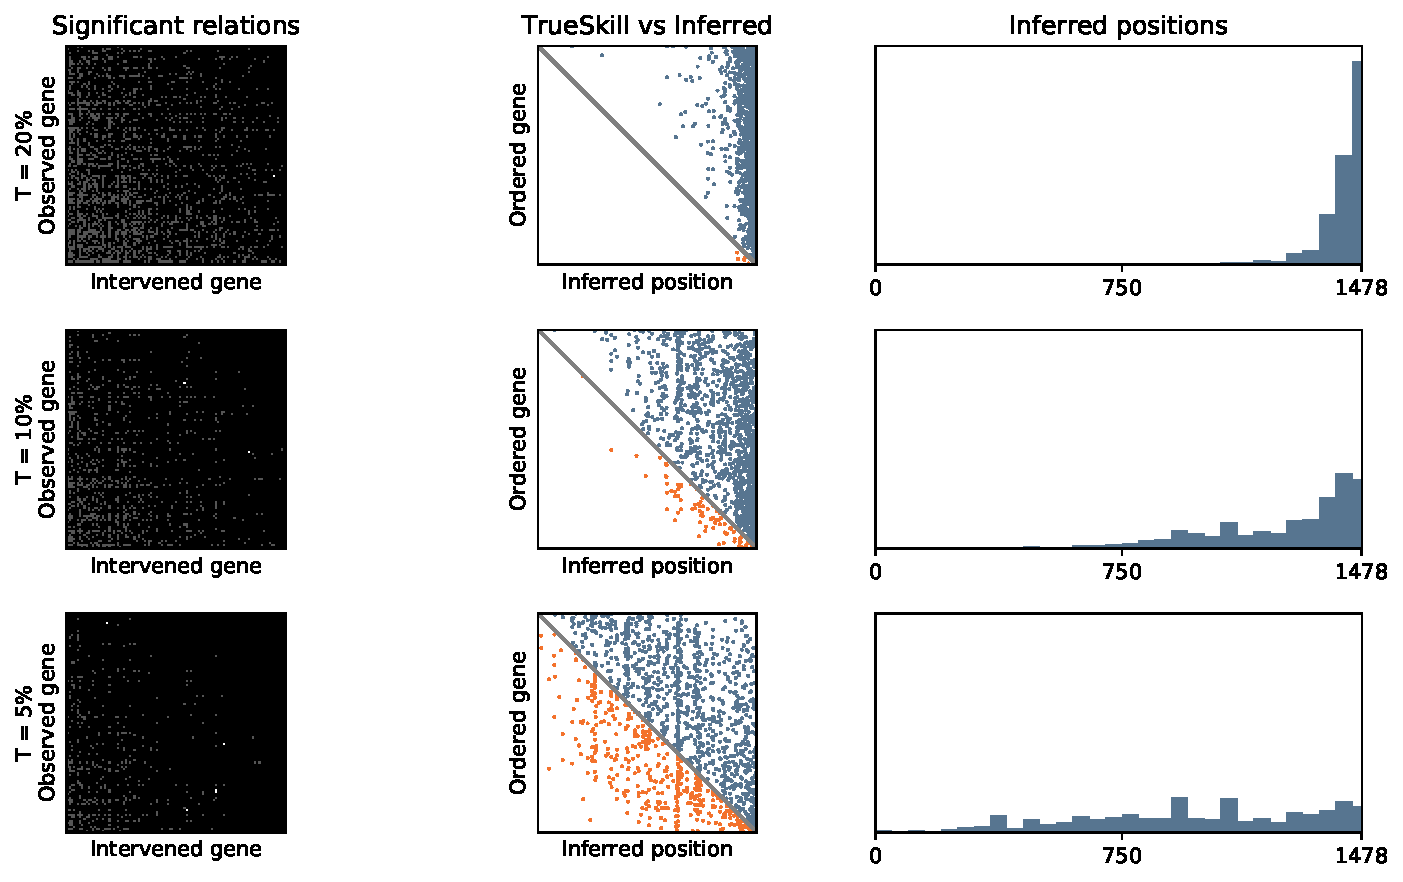
\includegraphics[width=\textwidth]{5inferred_positions.pdf}
    \caption{Analysis of test gene position inference for three different thresholds on the absolute expression values.}
    \label{fig:5:positions}
\end{figure}

Figure \ref{fig:5:positions} shows the results of the analysis for ground-truth thresholds $5\%$, $10\%$, and $20\%$. The left column shows the significant relations given the threshold, where the variables are ordered by the inferred order. Visually, for each gene on the rows, we look up the significant relation furthest to the right. The middle column shows only these last relations, and thus the estimated position for each gene. Note that if the order were correct, and no other order was possible (e.g. if the variables were on a Markov chain), the perfect positions would follow the gray diagonal line. Orange positions are estimated earlier in the order, blue positions later. The right column shows the distribution of estimated positions. 

% We choose threshold $10\%$ for our experiments. 
Threshold $5\%$ yields the nicest distribution of estimated positions. Many variables are placed at early positions compared to the results for higher thresholds. However, many of these early positions are earlier than their true position in the inferred order. This is not necessarily wrong, but we cannot verify this. If we make a lot of mistakes, the context becomes meaningless. We do not want to risk this. On the other hand, threshold $20\%$ estimates most positions to be far in the order. This means we approach the original context definition, since most interventions will be earlier than the estimated position of most genes. We choose threshold $10\%$ for our experiments as a good middle way.











% - How does the LCD method generally work?
%     - Why is it chosen? How does it generally perform? What is expected of it?
%     - On what assumptions does it rely?
%     - How is it proven?
%     - What statistical test is used?
% - How are the order-based and original context variables constructed?
%     - The puzzle of context construction
%     - Original C, graphical problem
%     - Order-based C, (still problematic?)
%     - Introduction to the problem of placing test genes in an order of train genes
%     - How is position inferred?
%     - Short analysis, justification of value threshold parameter
%     * something about 'detail', see notes Joris

% Somewhere:
% - L2 boosting preselection for speedup and great baseline (although not as good in other papers)

% Maybe:
% Note that the discrete nature of the variables and their relations makes the question of exogeneity nontrivial, and we do not provide any proofs here.

% \subsection{Local Causal Discovery}

% Local Causal Discovery has been proposed as a fast, incomplete algorithm to discover ancestral relations. The original formulation by \citet{cooper1997simple} depends on an underlying Bayesian Network and thus acyclicity. A more recent formulation by \citet{mooij2016joint} generalizes the algorithm to SCMs that allow cycles. 



% \subsubsection{Assumptions}

% The algorithm tests for a causal relation $X\to Y$ between two endogenous variables, using a third exogenous variable $C$ (the context). A small set of statistical independence tests restricts the set of possible causal subgraphs with $X$, $Y$ and $C$, and allowes us to infer under some circumstances that $X$ is an ancestor of $Y$. 

% LCD is based on the following assumptions:

% \begin{enumerate}
%     \item Underlying SCM (JCI-0)
%     \item Exogeneity of a context variable (JCI-1)
%     \item Causal faithfulness
%     \item Unbiased data selection
%     \item Independence oracle, and Dependence oracle
% \end{enumerate}



% \subsubsection{Statistical tests}

% LCD specifically discovers those causal relations, which effect can be measured from the data as $\Prb _M(Y|do(X=x)) = \Prb _M(Y|X=x)$. This is the case when only $X$ has an effect on $Y$ (i.e. no confounding or effect from $C$). Figure \ref{fig:5:lcdgraphs} shows the three subgraphs that satisfy this condition. Note that all possible relations between $C$ and $X$ given the exogeneity assumption are included.

% All subgraphs satisfy one independence and five dependence relations:

% \begin{enumerate}
%     \item $C \CI Y \given X $
%     \item $C \nCI X$
%     \item $X \nCI Y$
%     \item $C \nCI Y$ (follows from 2 and 3)
%     \item $X \nCI Y \given C$ (follows from 1 and 3)
%     \item $C \nCI X \given Y$ (follows from 1 and 2)
% \end{enumerate}

% The last three relations can be infered from the first three, using the causal faithfulness assumption and the Markov property. \citet{cooper1997simple} proved that the first three relations are sufficient to infer the causal relation $X\to Y$, by enlisting all possible subgraphs. 

% Most LCD implementations only check the first three relations. However, if assumptions are violated, some nonexistent causal relations might be infered. One can sacrifice recall for precision by testing some or all of the last three relations. \citet{cooper1997simple} warns specifically that the independence relation ($C \CI Y \given X$) is vulnerable to faithfulness violations, and suggests testing the fourth relation ($C \nCI Y$) as well. \citet{triantafillou2017predicting} aim for high precision and test all six relations.

% A common choice of dependence test is the two-tailed Fisher z-test \citep{fisher1924distribution}, which tests if the partial correlation is zero. Specifically, if we want to test $X \nCI Y \given Z$, we set the hypotheses:

% \begin{itemize}
%     \item[$H_0$:] $\rho_{XY|Z}=0$
%     \item[$H_A$:] $\rho_{XY|Z}\not = 0$
% \end{itemize}

% The partial correlation 

% z-transform -> test statistic z

% test hypothesis: p = 2*PHI(-sqrt... |z|)

% Pragmatic: use as independence test as well (different alpha, usually same value, but e.g. not in \citet{triantafillou2017predicting})


% SOMETHING ABOUT ASYMMETRY, but what was it and where did I read it?

